\chapter{Trabalhos Relacionados}

Nesta seção falaremos sobre trabalhos semelhantes à proposta de viagens solidárias. Selecionamos 5 aplicativos voltados para a área acadêmica ou desenvolvidos por grandes empresas como Waze e Blablacar. Ao final, apresentamos a tabela de comparação utilizando os recursos necessários para nossa área acadêmica e principalmente o fato de o aplicativo ser \textit{open-source}\footnote{Open-source: Ele é um código projetado para ser acessado abertamente pelo público: todas as pessoas podem vê-lo, modificá-lo e distribuí-lo conforme suas necessidades. Disponível em: <https://www.redhat.com/pt-br/topics/open-source/what-is-open-source> Acesso em: 26 de Nov. de 2021} e pode ser adaptado à realidade de nossa faculdade.

\section{Vemcar}
%Desenvolvido na Universidade Federal do Rio Grande do Norte, o aplicativo Vemcar começou a ser desenvolvido em uma disciplina oferecida no curso de Engenharia de Software, logo após, o protótipo passou para a equipe da Superintendência de Informática da Universidade Federal do Rio Grande do Norte (SINFO), lá foi realizado toda a validação da ideia, surgimento dos requisitos e foram aplicadas as regras do um processo de software. No Vemcar somentes pessoas ligadas à universidade( professores, alunos, técnicos) podem utilizar o aplicativo.
O aplicativo Vemcar foi desenvolvido no Universidade Federal do Rio Grande do Norte. Foi desenvolvido inicialmente como parte do curso de Engenharia de Software, antes de o protótipo ser entregue à equipe da Superintendência de Ciência da Computação do Universidade Federal do Rio Grande do Norte (SINFO), onde ocorreu toda a validação da ideia, a criação dos requisitos e a aplicação das regras de um processo de software. Na Vemcar, somente pessoas relacionadas a universidade (professores, alunos, técnicos) podem utilizar o aplicativo.

%texto escrito por mim

\begin{figure}[!hbtp]
	\centering
	\caption{Aplicativo de Carona Solidária Vemcar}
	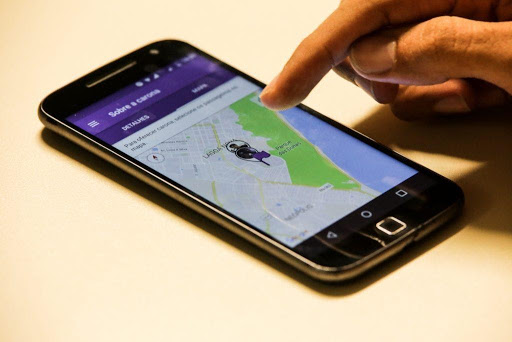
\includegraphics[width=0.6\textwidth]{./04-figuras/vemcar.jpg}
	\label{fig:tecnologia}
	\fonte{https://www.ufrn.br/imprensa/materias-especiais/2872/aplicativo-de-caronas-solidarias-da-ufrn-registra-mil-downloads-em-uma-semana}
\end{figure}

\section{RideUFF}

%O RideUFF é um projeto da Universidade Federal Fluminense - UFF motivado pelo problema de mobilidade urbana enfrentando pelos estudantes. Com o intuito de facilitar o trajeto dos academicos, o RideUFF quer oferecer também a economia, conforto, segurança e sustentabilidade (RideUFF). 
O RideUFF é um projeto da Universidade Federal Fluminense - UFF, motivado pela problemática da mobilidade urbana dos estudantes. Com o objetivo de facilitar a jornada dos acadêmicos, o RideUFF também visa proporcionar economia, conforto, segurança e sustentabilidade (RideUFF).

%A procura por vagas é grande na UFF e por muitas vezes os que buscam caronas não encontram aqueles que querem oferecer por causa da falta de centralização desse tipo de oferta. Há muitos grupos de Whatsapp onde são ofertadas caronas, deixando as ofertas dificeis pois para isso seria necessário os estudantes estarem em todos os grupos para encontrar uma carona que lhe atenda.
A procura por caronas é grande na UFF e muitas vezes quem procura carona não encontra as pessoas que desejam oferecer porque esse tipo de oferta não é centralizada. Existem muitos grupos de Whatsapp onde são oferecidas caronas compartilhadas. Isso dificulta as ofertas porque exigiria que os alunos estivessem em todos os grupos para encontrar uma carona adequada.

%O projeto se inspirou na iniciativa da UFRJ com o aplicativo Caronaê, também uma solução de mobilidade inteligente que foi implementado para centralizar as caronas ofertadas na universidade federal do rio de janeiro, o RideUFF tem a mesma intenção
O projeto foi inspirado por outras iniciativas de caronas universitárias, uma delas foi a da UFRJ com o aplicativo Caronaê, também uma solução de mobilidade inteligente implementada para centralizar as viagens oferecidas no Colégio Federal do Rio de Janeiro, o RideUFF tem a mesma intenção.

%\section{Caronaphone}


\section{Caronaê}

%mencionar trabalho da luísa e do artigo publicado sobre o aplcativo.

%O Caronaê é um aplicativo de carona voltada para o ambiente universitário desenvolvido por alunos da Universidade Federal do Rio de Janeiro (UFRJ). O aplicativo está disponível para duas plataformas, Android e iOS. Em seu site oficial (CARONAÊ, 2020) diz que \textit{“O Caronaê é um sistema de código aberto, seguro e prático de caronas compartilhadas, criado com o objetivo de ser replicado em diferentes instituições e feito exclusivamente para a comunidade acadêmica das instituições integrantes da Rede Caronaê”}.
O Caronaê é um aplicativo de carona desenvolvido por alunos da Faculdade Federal do Rio de Janeiro (UFRJ) e voltado para o ambiente universitário. O aplicativo está disponível para duas plataformas, Android e iOS. O site oficial afirma que Caronaê é um sistema de carona aberto, seguro e prático, desenvolvido com o objetivo de ser replicado em diferentes instituições e exclusivamente para a comunidade acadêmica das instituições que pertencem à rede Caronaê (CARONAÊ, 2020).

%Dos pontos interessantes que o aplicativo oferece são, o uso exclusivo da comunidade acadêmica, a centralização das ofertas de carona, o aumento da taxa de ocupação dos veículos e pontos de carona para facilitar o encontro de caroneiro e carona. A Figura~\ref{fig:caronae} mostra a tela inicial do site do aplicativo de carona \textbf{Caronaê}.
Os pontos de interesse oferecidos pelo aplicativo incluem uso exclusivo pela comunidade acadêmica, centralização da oferta de caronas, aumento da utilização de veículos e pontos de carona para facilitar o encontro de caronas e caroneiros. %Na Figura ~\ref{fig:caronae} temos a propaganda do aplicativo no site oficial. %podemos ver a tela inicial do aplicativo.mostra a tela inicial do site do aplicativo Caronaê.

\begin{comment}
\begin{figure}[!hbtp]
	\centering
	\caption{Aplicativo de Carona Solidária Caronaê}
	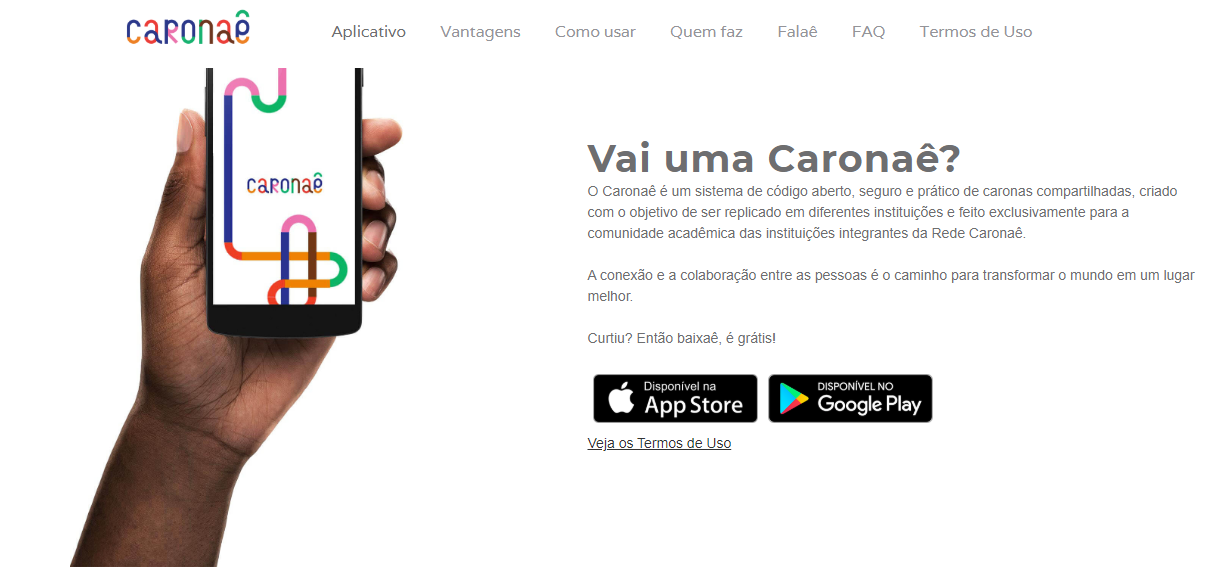
\includegraphics[width=0.8\textwidth]{./04-figuras/caronae.png}
	\label{fig:caronae}
	\fonte{https://caronae.org/index.html}
\end{figure}
\end{comment}

\section{Waze Carpool}
Aplicativo das Empresas Waze, o \textit{Waze Carpool} é uma variante dos serviços da Waze que oferece compartilhamento de caronas entre seus usuários. O serviço oferecido pela empresa funciona através de um programa de parcerias. O aplicativo é bem dinâmico e intuitivo. A empresa aproveita os dados do aplicativo Waze para alimentar a dinâmica de navegação do Waze Carpool. como mostra a tela de grupos do aplicativo na Figura~\ref{fig:tela_grupos_wazecarpool}.

\begin{figure}[!hbtp]
	\centering
	\caption{Tela de grupos do aplicativo Waze Carpool}
	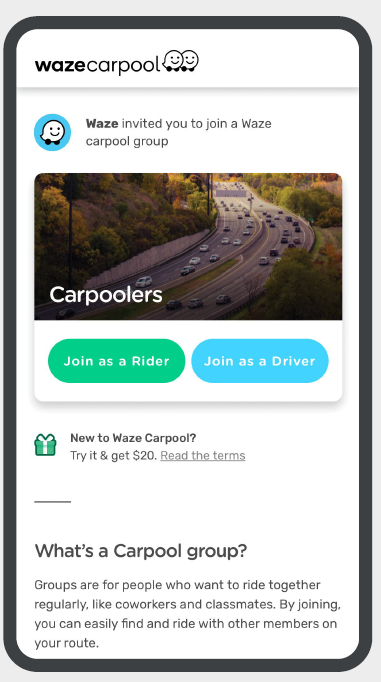
\includegraphics[width=0.3\textwidth]{./04-figuras/waze/Tela_de_grupos.png}
	\label{fig:tela_grupos_wazecarpool}
	\fonte{Programa de Parceria Brasil - Waze Carpool}
\end{figure}

%A Waze oferece o serviço do aplicativo para diversas empresas que desejam incorporar a cultura das caronas entre seus empregados porque a empresa acredita que as caronas costumam aproximar mais as pessoas e criar momentos que no local de trabalho não existiriam.
O Waze oferece um aplicativo para várias empresas que incorporam uma cultura de carona entre seus funcionários, pois a empresa acredita que a carona aproxima as pessoas e cria momentos que não existem no local de trabalho.

%O aplicativo tem uma dinâmica interessante, funciona a partir da criação de grupos, e os usuários destes grupos oferecem caronas entre si. Alunos de universidades como a UFRJ que por um tempo teve o seu próprio aplicativo de carona, o Caronaê, utilizam a ferramenta para pegar e oferecer a carona aos integrantes dos grupos que são criados e gerenciados por uma pessoa que ficar responsável pela comunicação da instituição com a empresa, o chamado "Embaixador".
O aplicativo tem uma dinâmica interessante, pois funciona criando grupos, e os usuários desses grupos oferecem caronas uns aos outros. %Estudantes de universidades como a UFRJ, que há algum tempo tinha um serviço próprio de carona, usam a ferramenta para pegar membros de grupos e oferecer carona. 
Esses grupos são criados e administrados por um responsável pela comunicação da instituição com a empresa, chamado de "embaixador".
% texto do material da waze 



\section{Quadro Comparativo}

\begin{quadro}[H]
	\centering
	\caption{Trabalhos Relacionados}
	\label{tab:quadro-comparativo}
	\resizebox{1.0\textwidth}{0.1\textheight}{
	\begin{tabular}{|l|c|c|c|c|c|}
		\hline
		& Caronaê & Vemcar & RideUFF & Waze Carpool & Blablacar \\ \hline
		Oferecer/Solicitar
		Caronas &         Sim       &     Sim  &   Sim      &     Sim        &   Sim                      \\ \hline
		Identificação dos 
		usuários &        Sim        &     Sim   &   Sim      &    Sim         &    Sim                     \\ \hline
		Restrição do público       &      Sim          &    Sim    &   Sim      &     Não        &       Não                  \\ \hline
		Remuneração            &      Não         &   Não   &   Não      &      Sim       &        Sim                 \\ \hline
		Plataforma                 &      Android/iOS          &   Android     &  Android       &      Android/iOS       &  Android/iOS                       \\ \hline
		Chat entre 
		usuários        &        Sim        &    Sim     &   Não      &      Sim       &       Sim                  \\ \hline
		Open-source        &      Sim          &    Não    &    Não     &      Não       &      Não                   \\ \hline
\end{tabular}
}
\end{quadro}

